\chapter{Valg av teknologi}
Dette kapitlet gjennomgår teknologien som ble valgt til å utvikle applikasjonen, teknologien som ble vurdert men ikke valgt og årsaken til valgene som ble gjort. For at applikasjonen skulle ha mulighet til å nå kravene spesifisert i kravspesifikasjonen var det viktig å vurdere nøye hvilke teknologier som passet best til den gitte problemstillingen.

\section{Utviklingsrammeverk}
Under valget av utviklingsrammeverk var det to faktorer som var spesielt viktig å ta med inn i vurderingen. De spesifikke kravene det siktes til er det funksjonelle kravet F1 beskrevet i tabell \ref{tbl:funksjonelle-krav} og det ikke-funksjonelle kravet IF2 beskrevet i tabell \ref{tbl:ikke-funksjonelle-krav}. F1 og IF2 handler henholdsvis om at utviklingsrammeverket må gjøre det mulig å implementere et kartgrensesnitt ved hjelp Kartverkets tjenester og at det skal være mulig å lage en kryssplattform applikasjon som skal fungere på både iOS og Android.

\subsection{Krav om en kryssplattform-applikasjon}
På bakgrunn av det ikke-funksjonelle kravet IF2 var det flere ulike utviklingsrammeverk som ble vurdert. Likt for alle rammeverkene som ble vurdert var det at de tilbyr utvikling av en applikasjon for både iOS og Android med bare én kodebase. Ved å bare ha én kodebase vil utviklingstiden kunne reduseres betraktelig ettersom at man slipper å lage den samme applikasjonen to ganger. Framtidig vedlikehold og oppdateringer vil også være lettere og raskere å utføre. Utviklingsrammeverkene som ble vurdert til applikasjonen var Flutter \cite{FlutterBeautifulNative} utviklet av Google, NativeScript \cite{NativeScript} som er et utviklingsrammeverk for kryssplattformutvikling med åpen kildekode, React Native \cite{ReactNativeFramework} laget av Facebook basert på JavaScript-rammerverket React \cite{ReactJavaScriptLibrary} og Ionic \cite{IonicCrossPlatformMobile} som er et kryssplattformrammeverk spesielt laget for mobile enheter. Alle disse ulike utviklingsrammeverkene tilbyr funksjonalitet for å lage en applikasjon for både iOS og Android med bare én kodebase. Likevel vil det alltid oppstå situasjoner hvor man er nødt til å skrive plattformspesifikk kode og disse situasjonene oppstår oftere hos noen rammeverk enn hos andre. Av de nevnte rammeverkene er Ionic det rammeverket som krever minst plattformspesifikk kode, mens React Native krever mest plattformspesifikk kode. Flutter og NativeScript havner en plass midt i mellom disse to \cite{FrameWorkComparison}. Ionic er også et av rammeverkene med flest ferdiglagde brukergrensesnitt-komponenter, noe som gjør at man under utvikling kan bruke mindre tid på grensesnittspesifikk implementasjon og mer tid på implementasjon av funksjonalitet. React Native har minst ferdiglagde komponenter mens Flutter stiller likt med Ionic. NativeScript havner en plass mellom Ionic og React Native \cite{FrameWorkComparison}.

\subsection{Krav om integrasjon med NorgesKart}
Det funksjonelle kravet F1 beskrevet i tabell \ref{tbl:funksjonelle-krav} beskriver at løsningen krever at kartet i applikasjonen bruker Kartverkets løsninger i form av tjenesten NorgesKart. Geonorge, som er det det nasjonale nettstedet for kartdata og annen stedfestet informasjon i Norge \cite{OmGeonorge}, linker til JavaScript-biblioteket Leaflet \cite{LeafletJavaScriptLibrary} i deres brukerveiledning om bruk av Kartverkets tjenester \cite{GeoNorgeLeaflet}. Også tidligere forsøk på implementasjon av en lignende applikasjon har brukt JavaScript-biblioteket Leaflet for å vise fram kartdata \cite[~s.116]{dystheEffektiviseringAvManuell2018}. For at implementasjonen av kartgrensesnittet i applikasjonen skulle gå så smertefritt som mulig ble det ble derfor tidlig bestemt at Leaflet skulle brukes. Derfor ble det viktig at utviklingsrammeverket støttet bruk av Leaflet. Flutter skrives i språket Dart \cite{FlutterDart} og støtter derfor ikke bruk av JavaScript-bibliotek Leaflet ettersom at Dart og JavaScript ikke er kompatible. Leaflet trenger direkte tilgang til et DOM-element \cite{IntroductionDOMWeb} for å legge selve kartet inn i brukergrensesnittet \cite{LeafletDom}. Selv om React Native skrives i språket JavaScript, støtter ikke React Native JavaScript-biblioteker som trenger direkte tilgang til DOM-elementer \cite{JavaScriptLibraryReactNative}. Det ble derfor ikke aktuelt å bruke hverken Flutter eller React Native i løsningen. Både Ionic og Native Script støtter bruk av JavaScript-rammerverket Angular \cite{IonicAngularOverview, NativeScriptAngular} for å lage brukergrensesnitt i applikasjonen. Angular støtter direkte tilgang til DOM-elementer \cite{AngularElementRef} i tillegg til at det støtter bruk av JavaScipt-bibliotek \cite{AngularJavaScriptLibraries}, noe som gjør at Leaflet vil fungere i både Ionic og NativeScript.

\subsection{Ionic + Capacitor}
Valget for hvilket utviklingsrammeverk som skulle brukes i applikasjonen falt til slutt på Ionic. Selv om NativeScript var en mulig kandidat, ble det bestemt å bruke Ionic ettersom at det potensielt kunne resultere i en mindre og lettere vedlikeholt kodebase og fordi Ionic har flere ferdiglagde brukergrensesnittkomponenter å velge mellom enn NativeScript \cite{FrameWorkComparison}. Ionic er en hybrid utviklingsplattform med åpen kildekode som kom på markedet i 2013 \cite{IntroducingIonicIonic}. Den gjør det mulig å lage kryssplattform-applikasjoner med web-teknologi og støtter de mest kjente JavaScript-rammerverkene som Angular, Vue.js og React, samt vanlig HTML, CSS og JavaScript \cite{IonicCrossPlatformMobile}. For at kode utviklet med web-teknologi skal kjøre på mobile eneheter og ha tilgang til maskinvare-funksjonalitet som mobilenes kamera eller GPS trengs det et mellomledd som binder sammen web-applikasjonen og maskinvaren \cite{CapacitorBlogHow}. Capacitor \cite{CapacitorCrossplatformNative} og Cordova \cite{ApacheCordova} er eksempler på slike mellomledd. Det ble besluttet å bruke Capacitor i utviklingen av denne applikasjonen. Årsaken til dette er at Capacitor er mer brukt, har 99\% bakoverkompatibilitet med utvidelser fra Cordova og fordi Capacitor kom ut i 2018 og bruker nyere moderne API-er som ikke var tilgjengelig da Cordova kom ut i 2009 \cite{CordovaVsCapacitor}. 

\begin{figure}[H]
\centering
\captionsetup{width=.8\linewidth}
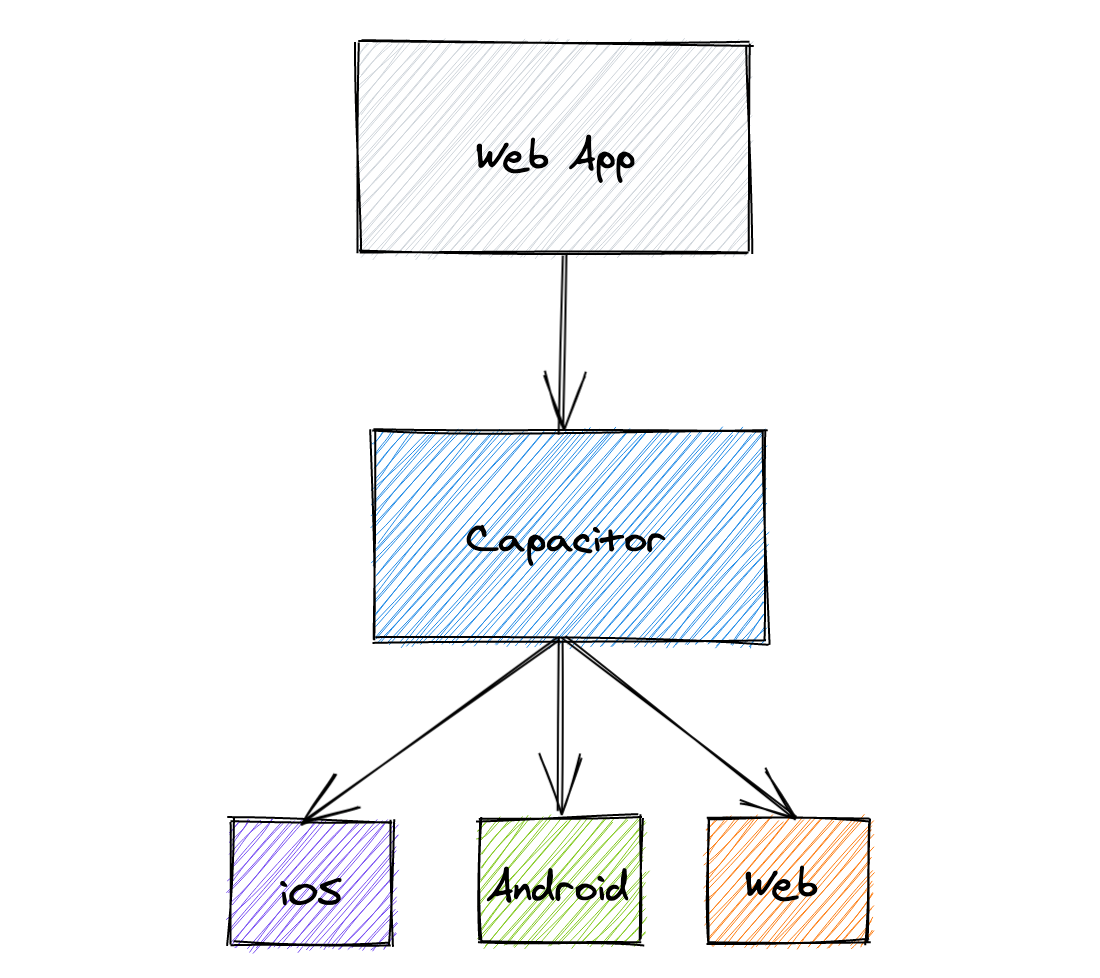
\includegraphics[scale=0.5]{Figurer/Bilder/capacitor-figure.png}
\caption{Forenklet figur som viser oppbygningen av en applikasjon som bruker web-teknologi sammen med Capacitor.}
\label{fig:how-capacitor-works}
\source{\cite{CapacitorBlogHow}}
\end{figure}

\section{Biblioteker}
\subsection{Frontend-bibliotek}
Ionic støtter bruk av flere forskjellige JavaScript-rammerverk for utvikling av web-applikasjon-delen av mobilapplikasjonen, samt støtte for vanlig HTML, CSS og standard JavaScript \cite{IonicCrossPlatformMobile}. JavaScript-rammeverkene som støttes per dags dato (17.03.2021) er Angular utviklet av Google \cite{Angular}, React utviklet av Facebook \cite{ReactNativeFramework} og Vue.js som er et uavhengig JavaScript-rammeverk med åpen kildekode \cite{VuejsVue2021}. Under utviklingen av litt større web-applikasjoner lønner det seg å bruke et JavaScript-rammeverk framfor å bruke standard HTML, CSS og JavaScript. Etterhvert som applikasjoner vokser kreves det flere filer og mer kode per fil. Å holde kontroll på disse på egenhånd ved hjelp av mapper og ryddig kode blir etterhvert vanskelig og kan føre til et spaghettilignende rot. De nevnte JavaScript-rammeverkene er laget for å holde koden i sjakk, gjøre det mulig å lage gjenbrukbare komponenter som fører til redusert kode og gir applikasjonen rom til å vokse mens den samtidig er lett å vedlikeholde \cite{aboutJavaScriptFrameworks}. En av ulempene med slike JavaScript-rammeverk er at de kan ha en relativt bratt læringskurve. Ettersom at begge prosjektdeltagerne hadde erfaring med utvikling med JavaScript-rammeverk fra før av ble denne problemstillingen ikke tatt i betraktning.
\newline

\noindent
Når det kom til valget av hvilket spesifikke rammeverk som skulle brukes stod det mellom React og Angular. Når applikasjonen ble påbegynt høsten 2020 var Ionic med Vue.js enda i Beta-versjon \cite{AnnouncingNewIonic} og ble derfor ikke sett på som et alternativ. Vi endte til slutt med å bruke Angular da Angular tilbyr strengere form for kodestruktur hvor HTML, CSS og JavaScript/TypeScript er delt opp i hver sin fil. Angular tilbyr også mulighet for å bruke TypeScript \cite{TypeScriptTypedJavaScript}, en versjon av JavaScript som gjør det mulig å typesette koden for økt struktur og enklere debugging \cite{AngularWhatAngular}.

\subsection{NGXS} \label{sub:ngxs}
Under planleggingen av applikasjonen ble det sett på som nødvendig å implementere en form for tilstandshåndtering for brukergrensesnittet. Applikasjonens flyt, spesielt under registrering av en saueflokk (se underkapittel \ref{subsubsec:registrering av sau} \nameref{subsubsec:registrering av sau}), består av flere ledd hvor å holde kontroll på antall registrerte søyer og lam med forskjellig farge, slips og øremerker er kritisk for at registreringen skal bli korrekt og brukeropplevelsen skal blir så bra som mulig. For å få til dette ble det valgt å bruke tilstandsbiblioteket NGXS \cite{IntroductionNGXS}. NGXS er modulert etter det populære tilstandsbiblioteket Redux laget for React, men reduserer redundant \textit{boilerplate}-kode ved å ta i bruk moderne TypeScript-funksjonalitet som klasser og dekoratører \cite{IntroductionNGXS}. Dataflyten ved bruk av NGXS illustreres i figur \ref{fig:ngxs-illustration}. Her referer \textit{Components} til ulike komponenter i brukergrensesnittet. \textit{Store} er den lagrede  tilstanden til applikasjonen, mens \textit{Actions} er handlinger utført av \textit{Components} som \textit{muterer} tilstanden i \textit{Store}. Når en komponent utfører en \textit{Action} og muterer en verdi i \textit{Store}, vil alle komponenter som tar i bruk den muterte verdien få beskjed om dette slik at komponentene får mulighet til å hente den siste tilgjengelige tilstanden. Applikasjonen består av flere ulike komponenter som har ansvaret for forskjellige funksjonalitet som for eksempel å lese opp tekst til brukeren under blind registrering (text-to-speech), ta i mot input fra brukeren eller vise hva som er registert i en oppsummering på skjermen. For at alle disse ulike komponentene skulle ha tilgang den samme informasjonen ble bruken av NGXS essensiell.
\begin{figure}[H]
\centering
\captionsetup{width=.8\linewidth}
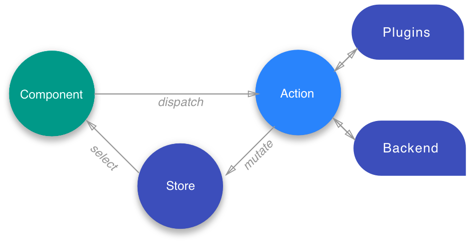
\includegraphics[scale=0.5]{Figurer/Bilder/ngxs-figure.png}
\caption{Dataflyt ved bruk av NGXS.}
\label{fig:ngxs-illustration}
\source{\cite{ngxsIllustration}}
\end{figure}

\subsection{Tekstopplesning}
For at applikasjonen skulle nå det funksjonelle kravet F4.1 \textit{Brukeren skal få verbale tilbakemeldinger om utførte handlinger underblind bruk slik at brukeren slipper å se på skjermen} beskrevet i tabell \ref{tbl:funksjonelle-krav} var det nødvendig å implementere en form for stemme som kunne gjengi informasjon vist på skjermen. Her sto valget mellom å enten bruke en tekstoppleser ofte brukt for blinde eller svaksynte, eller å spille inn en rekke lyder som kunne mikses og spilles av for å lese opp informasjon fra applikasjonen. Her falt valget på å bruke en tekstoppleser ettersom å spille inn lyder for hver eneste situasjon kom til å ta utrolig lang tid, samt at lydfilene ville brukt en del lagringsplass. Selv om dette kanskje ikke var tilfellet før har nå både iOS og Android innebygd støtte for tekstopplesning, ettersom at det gir økt tilgjengelighet for svaksynte og blinde \cite{TextToSpeechAndroidDevelopers, AVSpeechSynthesizerAppleDeveloper}. Det ville også gjort applikasjonen dårlig utrustet for eventuelle endringer eller utvidelser ettersom det da måtte brukes tid på spille inn nye lydfiler.
\newline

\noindent
Etter et forsøk på å implementere den sammfunnsutviklede Capacitor-utvidelsen \textit{capacitor-community/text-to-speech} \cite{CapacitorcommunityTexttospeech2021} i applikasjonen, kom det fram at den ikke hadde den funksjonaliteten som var ønsket for opplesing av tekst på iOS. For at brukeropplevelsen skulle bli så bra som mulig var det et behov for å kunne avbryte en tekst-opplesning før den var ferdig, og starte på opplesning av ny tekst. Dette fungerte utmerket på Android, men lot seg ikke gjøre i iOS med denne utvidelsen. Det ble derfor tatt en beslutning på å lage en egen utvidelse til Capacitor for tekstopplesning, ettersom at dette er sentral funksjonalitet i applikasjonen. Gjennom Capacitor er det heldigvis enkelt å utvikle og teste egne utvidelser både på Android og iOS \cite{CreatingCapacitorPlugins}. Utvidelsen \textit{capacitor-tts-plugin} ble laget for bruk i applikasjonen og er publisert på npmjs.com (\url{https://www.npmjs.com/package/capacitor-tts-plugin}), noe som gjør at man enkelt kan installere og bruke utvidelsen i sitt eget prosjekt ved hjelp av NPM \cite{NpmNpmDocs}. 


\section{Backend-løsning}
For at samhandling mellom brukere av applikasjonen skulle være mulig ble det behov for en form autentisering av brukere og sentral lagring av registrerte oppsynsturer. Det finnes mange ulike måter å gjøre dette på. Løsningene som ble vurdert for denne applikasjonen var enten Googles skybaserte løsning Firebase \cite{Firebase} eller en kombinasjon av rammeverket Node.js \cite{NodeJs} for å lage en tjener med MongoDB \cite{MongoDBAtlasCloud} som databaseløsning. Valget falt til slutt på Firebase da det er svært enkelt å bruke, ikke har behov for en tjener og tar seg av autentisering og lagring eksternt i skyen. Kombinasjonen av en dedikert tjener med en ekstern dokument-database som MongoDB kunne passet utmerket til prosjektet da det gir flere muligheter og større frihet. Likevel krever en slik løsning både mer midler i form av ekstra maskinvare for å rulle ut tjenerkoden på, samt ekstra tid for implementering. Det ble derfor sett på som mer hensiktsmessig å gå for Firebase.

\subsection{Firebase}
Firebase ble laget av Firebase Inc i 2011 \cite{FirebaseCrunchbaseCompany}, før det ble kjøpt opp av Google i 2014 \cite{GoogleAcquiresFirebase}. Firebase er en BaaS, Backend-as-a-Service, som gjør at man istedenfor å lage sin egen tjener-løsning/backend, har mulighet til å bruke tjenesten Firebase for alle tjener-relaterte oppgaver \cite{WhatBaaSBackendasaService}. Dette gjelder alt fra autentisering med Firebase Authentication, lagring med Cloud Firestore eller maskinlæring med Firebase Machine Learning \cite{FirebaseProducts}.

\subsubsection{Cloud Firestore}
For lagring av brukere, beitelag og registrerte oppsynsturer bruker applikasjonen Cloud Firestore. Cloud Firestore er en NoSQL-database som lagrer filer/dokumenter på JSON-format i skyen. Cloud Firestore lagrer data i en 3-delt struktur. \textit{Data}, i form av JSON, lagres i \textit{documents}, som igjen lagres \textit{collections}. En \textit{collection} kan ha en eller flere dokumenter, men et \textit{document} har også mulighet til å peke til nye \textit{collections} \cite{CloudFirestoreFirebase}. Systemet gjør det altså mulig å lagdele data som lagres i databasen for struktur og logikk. Dette var funksjonalitet som var nødvendig i vårt tilfelle ettersom vi ønsket å dele inn tilgang på registrerte oppsynstur basert på brukere og beitelag.
\begin{figure}[H]
\centering
\captionsetup{width=.8\linewidth}

\includegraphics[scale=0.4]{Figurer/Bilder/structure-data-firestore.png}
\caption{Datastruktur i Cloud Firestore.}
\label{fig:firestore-datastrktur}
\source{\cite{CloudFirestoreFirebase}}
\end{figure}

\subsubsection{Firebase Authentication}
Firebase Authentication er Firebase sin løsning for autentisering i skyen. Tjenesten støtter innlogging gjennom Facebook, Google, Twitter osv, men også innlogging med brukernavn og passord. Data for den innloggede brukeren lagres i skyen og brukes til autentisering når en bruker prøver å lese eller skrive til en fil i Cloud Firestore. Den eneste funksjonaliteten som trenger å bli implementert på selve enheten er en innloggings-side som sender brukernavn og passord til Firebase Authentication \cite{FirebaseAuthenticationSimple}. Ved å velge Firebase Authentication for autentisering ble en prosess som erfaringsmessig tar lang tid, gjort på bare én dag. Dette gjorde at vi kunne bruke mer tid på implementasjon av viktig funksjonalitet i andre deler av applikasjonen.

\section{Konklusjon}
For utvikling av selve grensesnittet ble utviklingsrammeverket Ionic sammen med JavaScript-rammeverket Angular valgt. Det ble her funnet ut at Ionic passet best for utvikling av denne applikasjonen basert på kravene presisert i kravspesifikasjonen. For å få tilgang til \textit{native}-funksjonalitet på mobiltelefonene applikasjonen skal kjøre på brukes Capacitor, da det var det mest moderne alternativet med mest funksjonalitet. Tilstandshåndteringen i applikasjonen tas hånd om av biblioteket NGXS, da det er laget for Angular og krever mindre \textit{boilerplate}-kode en tilsvarende bibliotek. For at applikasjonen skulle håndtere tekst-opplesning likt på både iOS og Android ble det utviklet en egen utvidelse til Capacitor for tekstopplesning som nå ligger ute i NPM-registeret for enkel bruk. Backend-løsningen i applikasjonen er gjort med en Backend-as-a-Service i form av Firebase, da det tilbyr all ønsket funksjonalitet mens det samtidig ga kortest mulig implementasjonstid.